% Copyright 2009--2010  Ed Bueler

\begin{frame}{notation} 

\begin{center}
  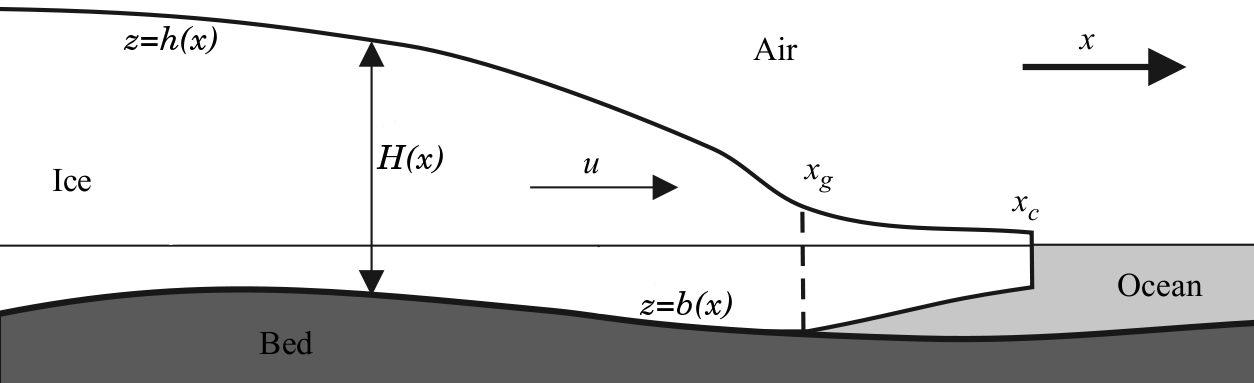
\includegraphics[width=0.8\textwidth]{photos/flowline}

\vspace{-0.1in}
\tiny \emph{figure modified from} [Schoof, 2007]\nocite{SchoofMarine1} \normalsize
\end{center}

\scriptsize
  \begin{itemize}
  \item coordinates $t,x,y,z$ \hfill  ($z$ is vertical, positive upward)
  \item subscripts for partial derivatives: $u_x = \partial u/\partial x$
  \item $h=$ ice surface elevation, \quad $b=$ bedrock elevation
  \item $H=$ ice thickness
  \item $T=$ ice temperature
  \item $(u,v,w)=$ ice velocity
  \item $\rho=$ density of ice, \quad $\rho_w=$ density of ocean water
  \item $g=$ acceleration of gravity
  \item $\strainrate_{ij}=$ strain rate tensor
  \item stress tensors: $\sigma_{ij}=$ Cauchy and $\tau_{ij}=$ deviatoric
  \item \alert{please ask about notation!} \qquad \scriptsize \dots there are no stupid questions \small
  \end{itemize}

\emph{notation here is generally consistent with  [Bueler and others, 2005]\nocite{BLKCB}, [Bueler and Brown, 2009]\nocite{BBssasliding}, [Fowler, 1997]\nocite{Fowler}, [Greve and Blatter, 2009]\nocite{GreveBlatter2009}, [Schoof, 2006; 2007]\nocite{SchoofStream,SchoofMarine1}}
\end{frame}


\begin{frame}{scope}

slogans:
  \begin{itemize}
  \item \alert{my focus is on approximating ice flow}
  \item \alert{my example numerical codes actually work}
  \end{itemize}
\medskip

continuum models:
  \begin{itemize}
  \item shallow ice approximation (SIA) in 2D
  \item shallow shelf approximation (SSA) in flowline (1D)
  \item mass continuity \& surface/base kinematical equations
  \item \dots and a little bit more
  \end{itemize}

\medskip
numerical ideas:
  \begin{itemize}
  \item finite difference schemes
  \item solving algebraic systems arising in stress balances
  \item verification
  \end{itemize}
\end{frame}


\begin{frame}{outside of scope}
\large\emph{not} \normalsize covered here:
  \begin{itemize}
  \item thermomechanical coupling
  \item subglacial material/process modeling
  \item snow/firn process modeling
  \item earth deformation
  \item numerical solution of Stokes equations
  \item grounding line and calving front issues
  \item anisotropy in ice flow
  \item paleoclimate modeling and ``spin-up''
  \item finite element, spectral, wavelet, multigrid, \dots methods
  \item \dots etc.~etc.
  \end{itemize}
\end{frame}


\begin{frame}{main equations}

\begin{itemize}
\item shallow ice approximation (SIA), equation \eqref{sia}
\item heat equation \eqref{heat} \quad\small\emph{(for analogy purposes)} \normalsize
\item surface kinematical equation \eqref{surfkine}
\item basal kinematical equation \eqref{basekine}
\item map-plane mass continuity equation \eqref{masscontinuity}
\item Stokes equations in a flow line, equations \eqref{Stokes}
\item shallow shelf approximation (SSA), equation \eqref{ssa}
\end{itemize}
\end{frame}


\begin{frame}{\textsc{Matlab}/\textsc{Octave} codes}

\begin{itemize}
\item these lectures are structured around
  \begin{itemize}
    \item 7 codes which solve PDEs
    \item an additional 13 codes which plot, pre-process, post-process
  \end{itemize}
\item \emph{each PDE code is 1/2 to 1 page in length}
\item all tested in \Matlab \scriptsize(v.~7.9) \normalsize and \href{http://www.gnu.org/software/octave/}{\Octave} \scriptsize(v.~3.2)\normalsize
\item available as
  \begin{itemize}
    \item[$\circ$] \texttt{.zip} or \texttt{.tar.gz}, from my USB memory stick, or
    \item[$\circ$] online:  \bigskip\small
      \centerline{\fbox{\url{http://www.dms.uaf.edu/~bueler/karthaus/}}}
  \end{itemize}
\end{itemize}
\end{frame}


\section[ice flow: a superficial view]{ice flow: an outsider's superficial view}

\begin{frame}{my first goal}

\begin{itemize}
\item I want to get to an equation for which I can say:
\bigskip

\begin{center}
\emph{numerically solve this equation, and you've got a usable model for} \dots (a specific ice flow problem) 
\end{center}
\bigskip

\item to get to that goal: I will \emph{very quickly} recall the continuum mechanics of ice flow
\item \dots from a naive outside view
\end{itemize}
\end{frame}


\begin{frame}{let's treat ice in glaciers as a \emph{fluid}}

\begin{itemize}
\item we describe fluids primarily by a \emph{velocity field} $\mathbf{u}(t,x,y,z)$
\item if the ice fluid were much faster-moving than it actually is\footnote{if gravity were a lot stronger and/or ice were a lot weaker, for example}, and if it were linearly-viscous like liquid water, then ice flow modeling would be more familiar to other the climate-modeling and/or engineering computational fluids people
\item \dots we would all use the Navier-Stokes equations, for incompressible fluids, as our flow model:
\begin{align*}
\nabla \cdot \mathbf{u} &= 0 &&\text{\emph{incompressibility}} \\
\rho \left(\mathbf{u}_t + \mathbf{u}\cdot\nabla \mathbf{u}\right) &= -\nabla p + \nu \nabla^2 \mathbf{u} + \rho \mathbf{g} &&\text{\emph{force balance}}
\end{align*}
\end{itemize}
\end{frame}


\begin{frame}{\emph{hmmm} \dots \emph{does not sound like glaciology to me!}}

is numerical ice flow modeling actually computational fluid dynamics?

\begin{itemize}
\item \alert{yes}
\item at geophysical scale like atmosphere/ocean
\item \dots but it is a weird one
\item consider what makes atmosphere/ocean flow modeling exciting:
  \begin{itemize}
  \item[$\circ$] turbulence
  \item[$\circ$] convection
  \item[$\circ$] coriolis force
  \item[$\circ$] density/salinity stratification
  \item[$\circ$] lots of tracers \& chemistry ($CO_2$, methane, ozone, \dots)
  \end{itemize}
\item none of the above list is relevant to ice flow!
\item so what could be interesting about the flow of slow, cold, shallow, non-turbulent, chemically-dull, old ice?
\end{itemize}
\end{frame}


\begin{frame}{ice is a slow, shear-thinning fluid}

\begin{itemize}
\item our fluid is

\phantom{foo bar}
  \begin{tabular}{lc}
  \emph{slow}: & $\rho \left(\mathbf{u}_t + \mathbf{u}\cdot\nabla \mathbf{u}\right) \approx 0$ \\
  \emph{non-Newtonian}: & viscosity $\nu$ is not constant in ``$\tau_{ij} = 2 \nu D_{ij}$''
  \end{tabular}
\item and so the standard ``full'' model for ice flow is shear-thinning Stokes as follows:
\begin{align*}
\nabla \cdot \mathbf{u} &= 0 &&\text{\emph{incompressibility}} \\
0 &= - \nabla p + \nabla \cdot \tau_{ij} + \rho \mathbf{g} &&\text{\emph{force balance}} \\
D_{ij} &= A \tau^{n-1} \tau_{ij} &&\text{\emph{flow law}}
\end{align*}
\item equations above are true at every instant, and so
  \begin{quote}
  \emph{geometry and boundary stress and ice strength determine velocity instantaneously} in the model
  \end{quote}
\end{itemize}
\end{frame}


\begin{frame}{ice is a slow fluid 2}

\begin{itemize}
\item the ``slow'' fact, $\rho \left(\mathbf{u}_t + \mathbf{u}\cdot\nabla \mathbf{u}\right) \approx 0$, means no forces of inertia from acceleration
\item thus velocity is \emph{not} a state variable of any model for evolving ice sheets and glaciers
\item \dots it is a ``diagnostic'' output \dots but a very important output!
\item an ice sheet code usually recomputes the full velocity field at every time, without storing it from the previous step\footnote{Bob Dylan would say: \emph{you don't need a glaciologist to remember which way the wind blows}}
\item to see how glacier flow fields change in time we must track the changes to
  \begin{itemize}
    \item[$\circ$] the location of the ice surface and base
    \item[$\circ$] the force (stress) applied at the boundary
    \item[$\circ$] the ice strength, as it changes with ice temperature (for example)
  \end{itemize}
\end{itemize}
\end{frame}


\begin{frame}{plane flow Stokes}

more concretely, the shear-thinning Stokes model is this:

\begin{itemize}
\item in the $x,z$ plane flow case the Stokes equations say
\begin{empheq}[]{align}
u_x + w_z &= 0 &&\text{\emph{incompressibility}}\notag \\
p_x &= \tau_{11,x} + \tau_{13,z} &&\text{\emph{stress balance} ($x$)} \notag \\
p_z &= \tau_{13,x} - \tau_{11,z} - \rho g &&\text{\emph{stress balance} ($z$)} \notag \\
u_x &= A \tau^{n-1} \tau_{11} &&\text{\emph{flow law} (diagonal)}\notag \\
u_z + w _x &= 2 A \tau^{n-1} \tau_{13} &&\text{\emph{flow law} (off-diagonal)} \notag
\end{empheq}
\item five equations in five unknowns ($u,w,p,\tau_{11},\tau_{13}$)
\item complicated enough \dots can I make it familiar by looking at a very-simplified situation?
\end{itemize}
\end{frame}


\begin{frame}{slab-on-a-slope}

\vspace{-0.05in}
\small

\begin{columns}
\begin{column}{0.5\textwidth}
\begin{itemize}
\item rotated coordinates: $\mathbf{g} = g \sin\theta\, \hat x - g \cos \theta \,\hat z$
\end{itemize}
\end{column}
\begin{column}{0.5\textwidth}
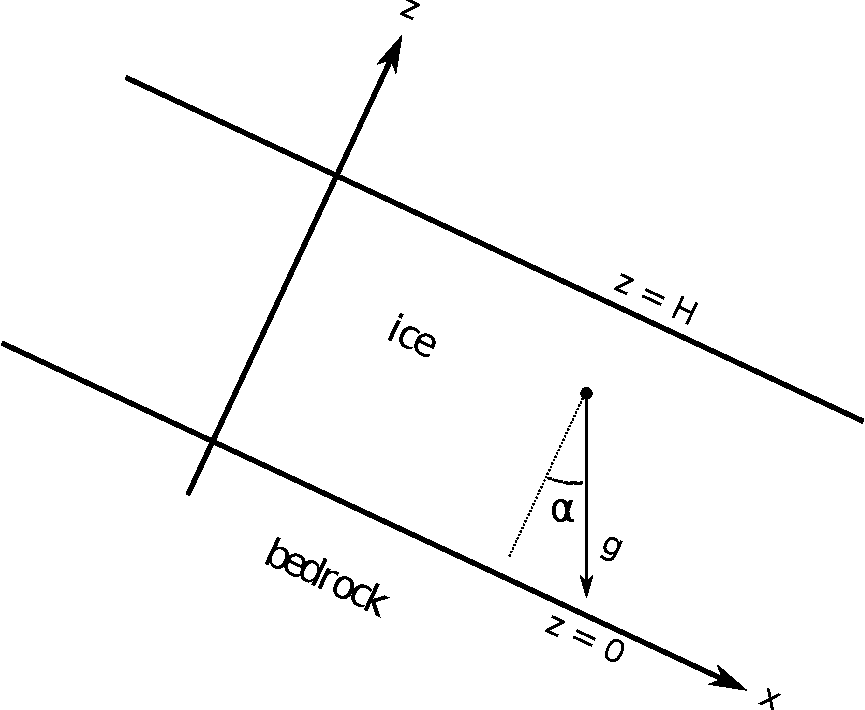
\includegraphics[width=1.0\textwidth]{photos/slab}
\end{column}
\end{columns}
\vspace{-0.2in}

\begin{itemize}
\item as on previous slide, but with $n=3$:
\small
\begin{empheq}[]{align}
u_x + w_z &= 0 &   u_x &= A \tau^2 \tau_{11} \notag \\
p_x &= \tau_{11,x} + \tau_{13,z} + \rho g \sin\theta &   u_z + w _x &= 2 A \tau^2 \tau_{13} \notag \\
p_z &= \tau_{13,x} - \tau_{11,z} - \rho g \cos\theta \notag
\end{empheq}
\small
\item \emph{but} for a slab-on-a-slope, by definition, there is no variation in $x$:
\small
\begin{empheq}[]{align}
w_z &= 0 &   0 &= \tau_{11} \notag \\
\tau_{13,z} &= - \rho g \sin\theta &   u_z &= 2 A \tau^2 \tau_{13} \notag \\
p_z &= - \rho g \cos\theta \notag
\end{empheq}
\end{itemize}
\end{frame}


\begin{frame}{slab-on-a-slope 2}

\small
\begin{itemize}
\item add some boundary conditions:
	$$w(\text{base})=0, \qquad p(\text{surface})=0, \qquad u(\text{base})=u_0,$$
\item further-simplified equations:
\begin{align*}
\tau_{13} &= \rho g \sin\theta (H-z) &  p &= \rho g \cos\theta (H-z) \\
w &= 0  & \tau_{11} &= 0
\end{align*}
\item and 
\vspace{-0.2in}
\begin{align*}
u(z) &= u_0 + 2 A (\rho g \sin\theta)^3 \int_0^z (H-z')^3\,dz' \\
     &= u_0 + \frac{1}{2} A (\rho g \sin\theta)^3  \left(H^4 - (H-z)^4\right)
\end{align*}

\vspace{-0.1in}
\end{itemize}
\begin{center}
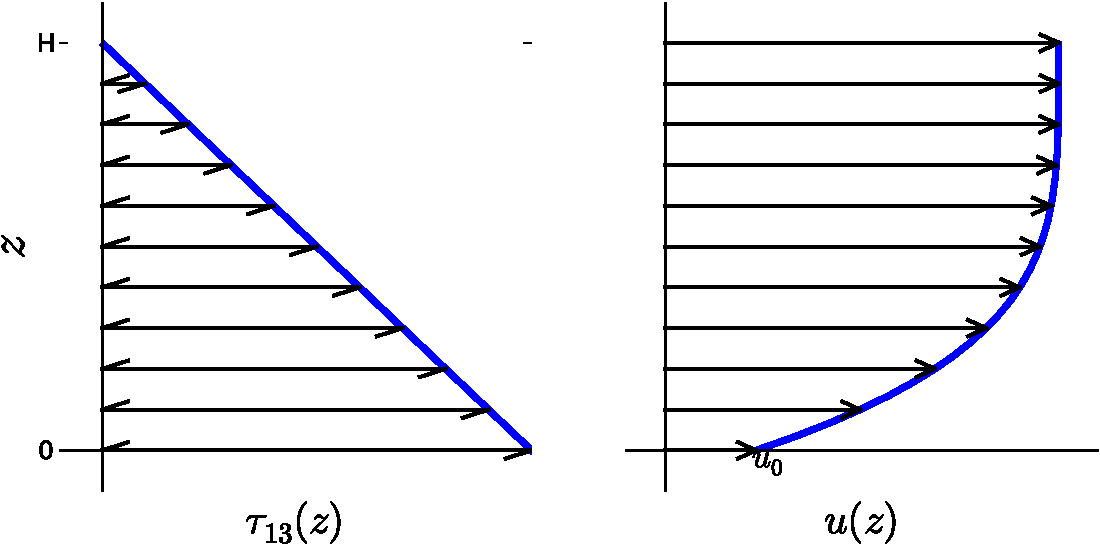
\includegraphics[width=0.6\textwidth]{photos/slabfigs}
\end{center}
\end{frame}


\begin{frame}{slab-on-a-slope 3}

\begin{columns}
\begin{column}{0.6\textwidth}
\begin{itemize}
\item do we believe these equations?
\item velocity on last slide (and below) was from a \emph{formula}
\item compare to observations at right
\item seems there is an element of truth
\end{itemize}
\begin{center}
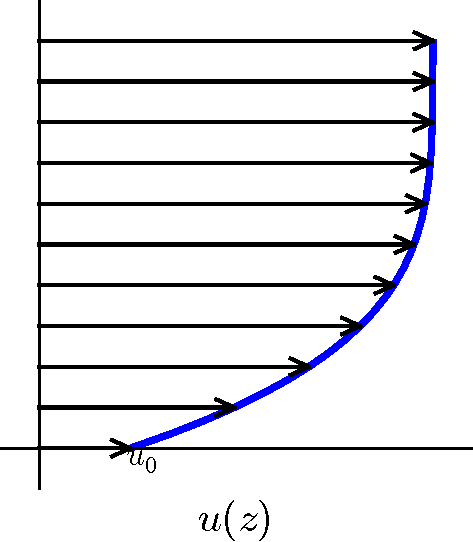
\includegraphics[width=0.4\textwidth]{photos/slabvel}
\end{center}
\end{column}
\begin{column}{0.4\textwidth}
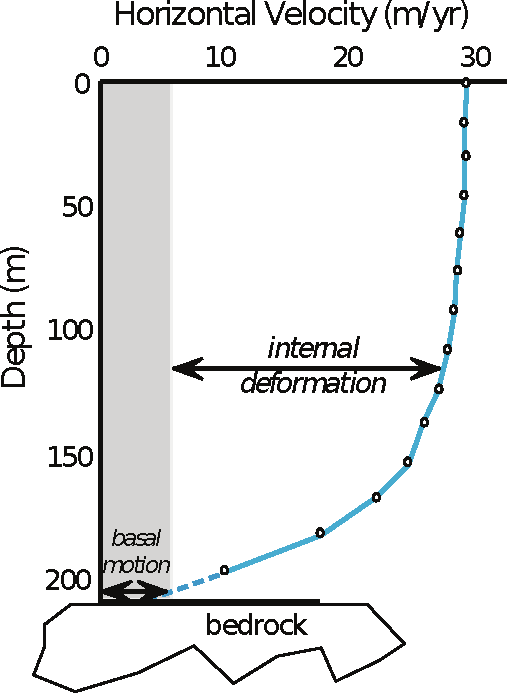
\includegraphics[width=0.9\textwidth]{photos/athabasca_deform}

\medskip
\scriptsize
Velocity profile of the Athabasca Glacier, Canada, derived from inclinometry.  [Savage and Paterson, 1963]\nocite{SavagePaterson}
\end{column}
\end{columns}
\end{frame}


\begin{frame}{mass continuity}

\small
now we know the velocity $u(z)$ \dots so what?
\begin{itemize}
\item suppose now that our slab has \emph{slowly varying thickness} $H(t,x)$
\item compute the vertical average of velocity, which depends on $x$:
	$$\bar u(x) = \frac{1}{H}\int_0^{H} u(x,z)\,dz$$
\end{itemize}

\begin{columns}
\begin{column}{0.6\textwidth}
\begin{itemize}
\item consider change of area (really: ice volume) in the figure at right:
	$$\frac{dA}{dt} = \int_{x_1}^{x_2} M(x)\,dx + \bar u_1 H_1 - \bar u_2 H_2$$
\item in limit where width $dx=x_2-x_2$ is small we have $A\approx dx\, H$
\item divide by $dx$ and get
   $$H_t = M - \left(\bar u H\right)_x$$
\item this is the \emph{mass continuity equation}
\end{itemize}
\end{column}
\begin{column}{0.4\textwidth}
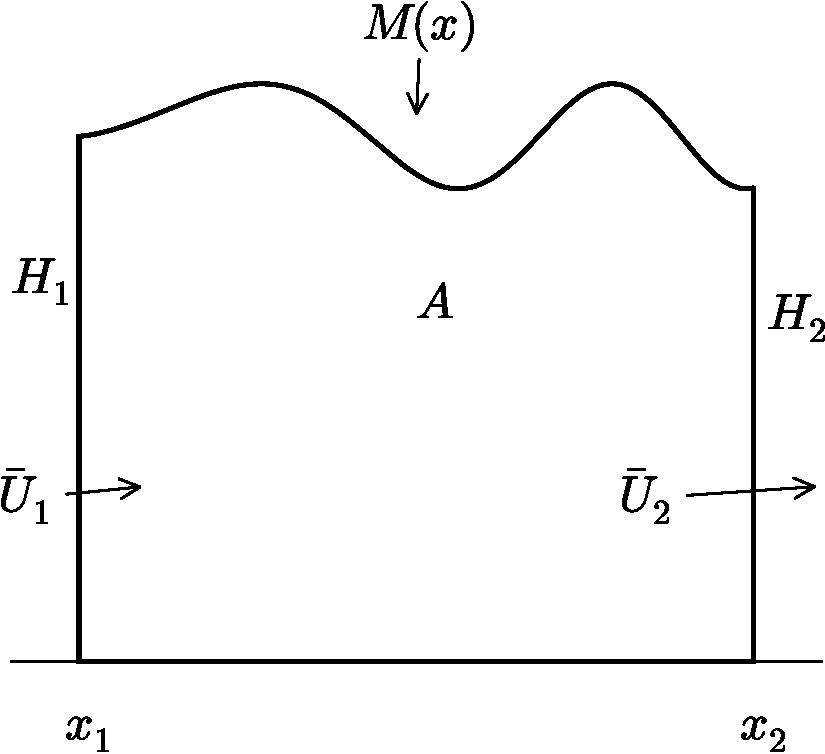
\includegraphics[width=1.0\textwidth]{photos/slabmasscontfig}
\end{column}
\end{columns}
\end{frame}


\begin{frame}{rough explanation of ``shallow ice approximation'' (SIA)}

\small
\begin{itemize}
\item I'll consider only $u_0=0$ case in these lectures (``non-sliding SIA'')
\item from slab-on-slope velocity formula,
\begin{align*}
\bar u H &= \int_0^H \frac{1}{2} A (\rho g \sin\theta)^3  \left(H^4 - (H-z)^4\right)\,dz \\
	&= \frac{1}{2} A (\rho g \sin\theta)^3  \left(\frac{4}{5} H^5\right) \\
	&= \frac{2}{5} A (\rho g \sin\theta)^3 H^5
\end{align*}
\item note $\sin \theta \approx \tan\theta = - h_x$
\item combine with mass continuity $H_t = M - \left(\bar u H\right)_x$:
\begin{equation}
H_t = M + \left(\frac{2}{5} A (\rho g)^3 H^5 |h_x|^2 h_x\right)_x  \tag{0}
\end{equation}
\item \emph{it is pretty rough \dots but we will get back to it}
\end{itemize}
\end{frame}


\begin{frame}{slow, non-Newtonian, shallow}

\begin{itemize}
\item ice sheet flow problems have three outstanding properties:
  \begin{enumerate}
  \item slow
  \item non-Newtonian
  \item shallow
  \end{enumerate}
\item all three properties will be in all of my models
\item regarding ``shallow,'' here in \alert{red} is a to-scale cross section of Greenland at $71^\circ$:
\begin{center}
  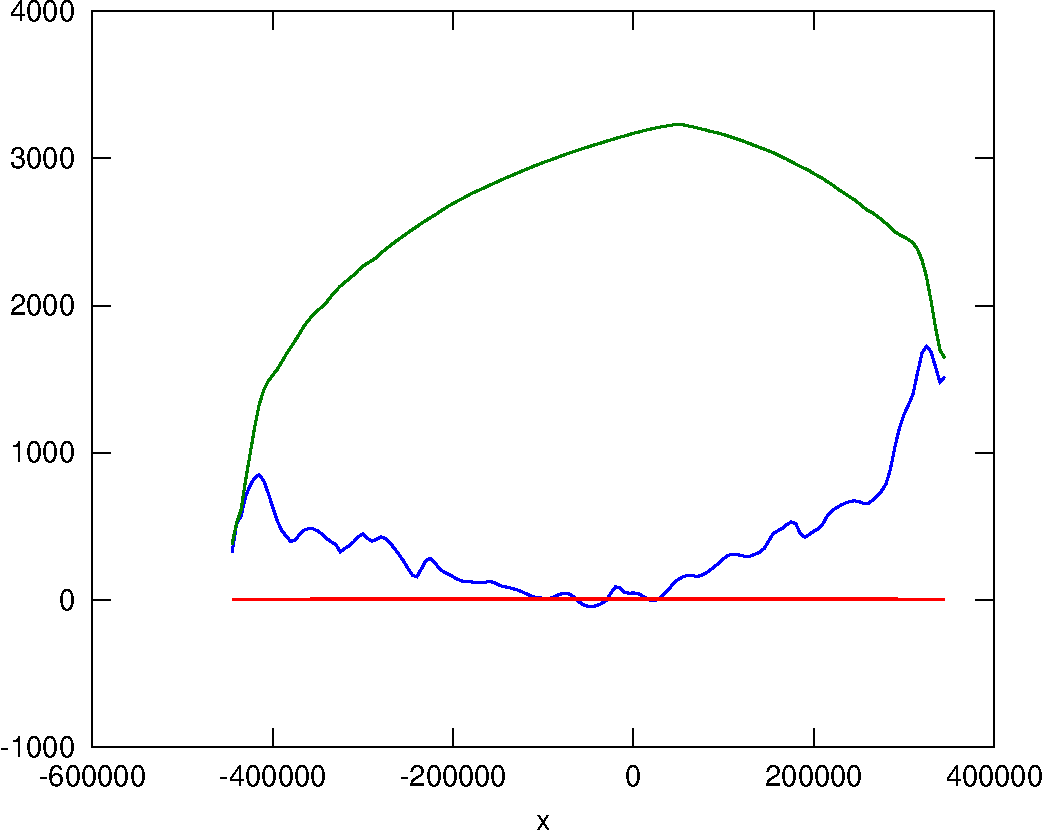
\includegraphics[width=0.6\textwidth]{photos/green_transect}
\end{center}
\end{itemize}
\end{frame}


\subsection{shallow ice approximation (SIA)}

\begin{frame}{the isothermal shallow ice approximation (SIA)}

is a model which applies reasonably well to
\begin{itemize}
\item grounded ice sheets
\item on relatively uninteresting bed topography, whose flow is
\item not dominated by sliding nor by liquid water at base or margin
\begin{center}
  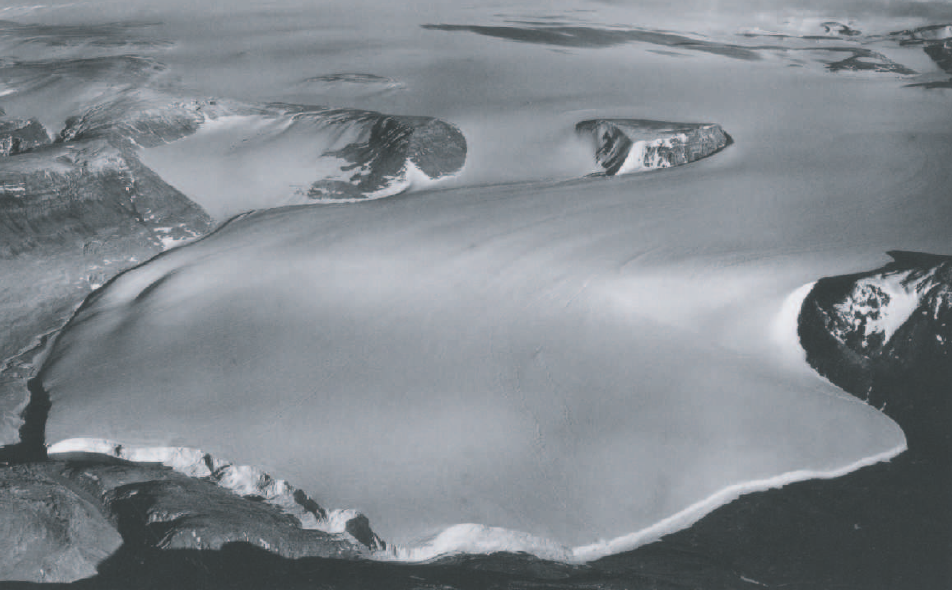
\includegraphics[width=0.7\textwidth]{photos/polaris}

\tiny ``Polaris Glacier,'' northwest Greenland, photo 122, [Post and LaChapelle, 2000]\nocite{PostLaChapelle}
\end{center}
\item might apply to the above
\end{itemize}
\end{frame}


\begin{frame}{isothermal shallow ice approximation 2}

\begin{itemize}
\item the non-sliding isothermal SIA:
\begin{empheq}[box=\fbox]{equation}
H_t = M + \Div \left(\Gamma H^{n+2} |\grad h|^{n-1} \grad h \right) \label{sia}
\end{empheq}
  \begin{itemize}
  \item[$\circ$] generalizes slab-on-slope equation (0) earlier
  \item[$\circ$] $h=H+b$
  \item[$\circ$] accumulation if $M>0$, ablation if $M<0$
  \item[$\circ$] recall Glen flow law: $\strainrate_{ij} = A(T) \devstress^{n-1} \devstress_{ij}$
  \item[$\circ$] $\Gamma$ is a positive constant
  \end{itemize}
\item \begin{minipage}[t]{2.5in}\emph{numerically solve equation \eqref{sia}, and you have a usable model for ice flow in the Barnes Ice Cap} [Mahaffy, 1976]\nocite{Mahaffy}\end{minipage}
\, \begin{minipage}[t]{1.1in}\vspace{-10pt}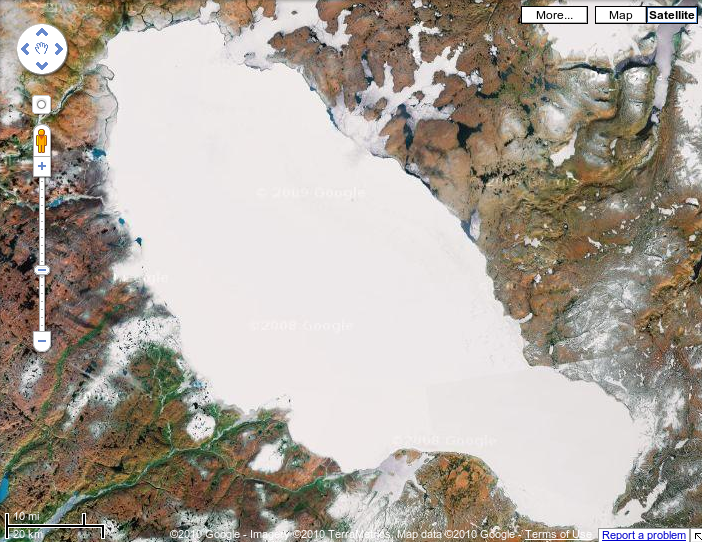
\includegraphics[width=1.0in]{photos/barnes}\end{minipage}
\item questions:
  \begin{itemize}
     \item[$\circ$] where does equation \eqref{sia} come from?
     \item[$\circ$] how to solve it numerically?
     \item[$\circ$] how to \emph{think} about it?
  \end{itemize}
\end{itemize}
\end{frame}
